\appendix
\chapter{User manual}

Due to this application being entered as a practical demonstration running on a Raspberry Pi board, this manual
provides the information necessary in the end to end preparation of the demo. This will help in correctly
setting up the Raspberry Pi, building and installing the application, and understanding the features
provided by the application.

\section{Raspberry Pi Setup}

\begin{figure}[H]
	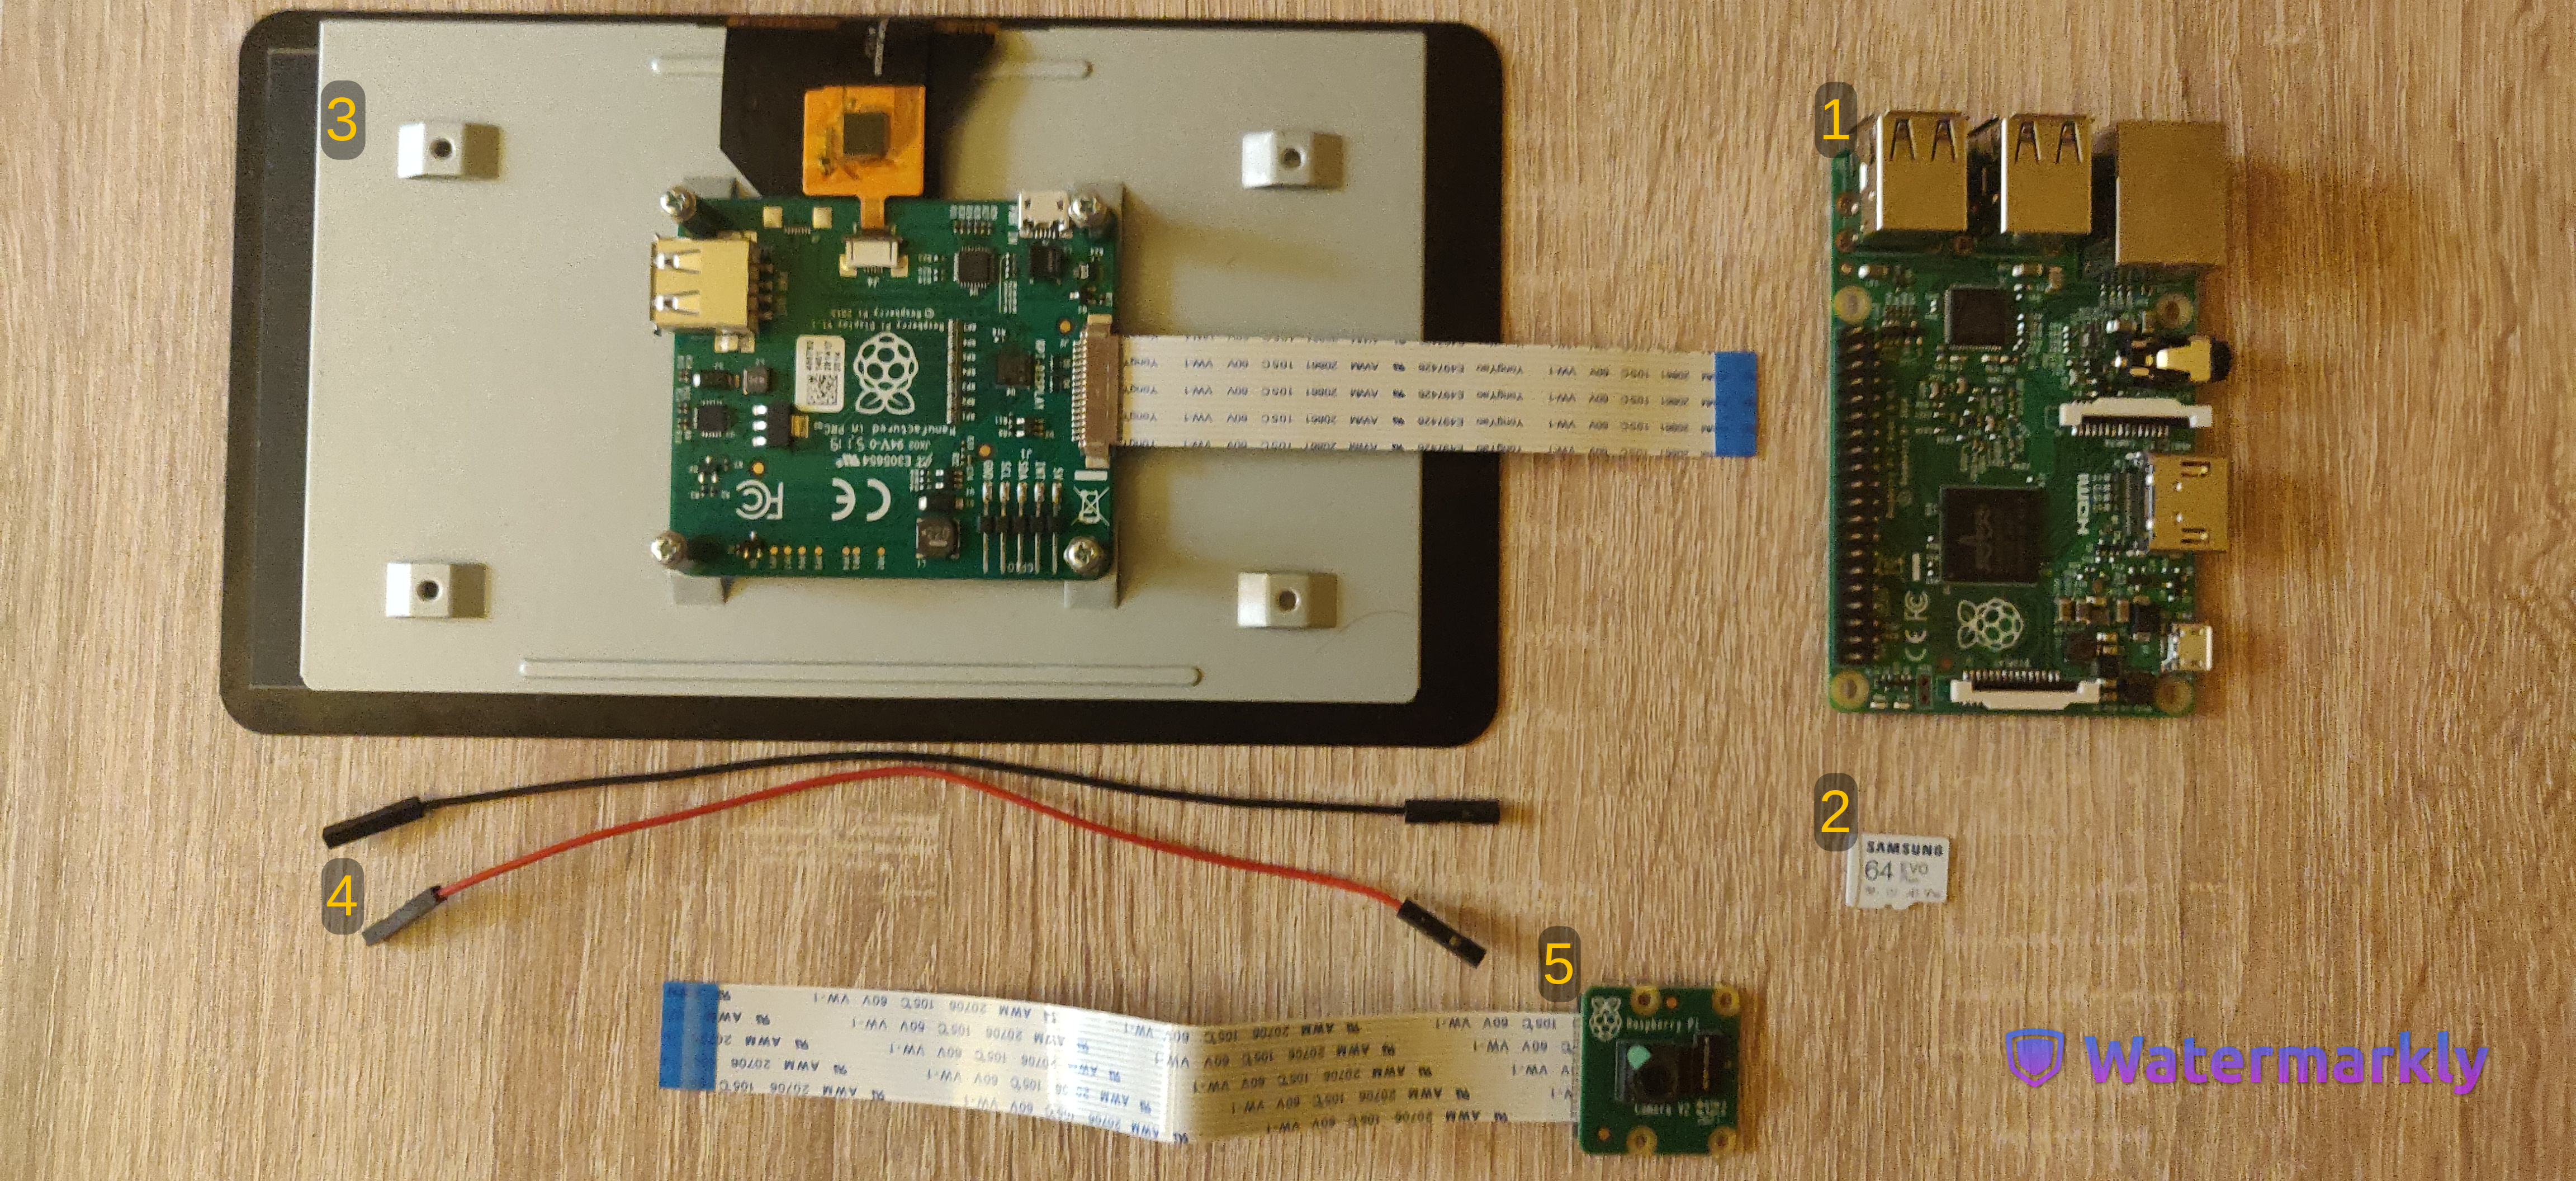
\includegraphics[width=0.95\textwidth, height=0.5\textwidth]{resources/Manual_Components.jpg}
	\caption{Required components}
\end{figure}

Those components are, in order:
\begin{enumerate}
	\item Raspberry Pi development board.
	\item SD card for storing operating system.
	\item Raspberry Pi Display, with ribbon cable attached.
	\item Jumper wires for powering display.
	\item Raspberry Pi Camera Module, with ribbon cable attached.
\end{enumerate}

Before proceeding with connecting the components, make sure a valid Debian-based operating system is installed
on the SD card. This can be achieved using the methods described within the Raspberry Pi documentation:
\url{https://www.raspberrypi.com/documentation/computers/getting-started.html#installing-the-operating-system}.

The following highlighted ports are used to connect the display and the camera:

\begin{figure}[H]
	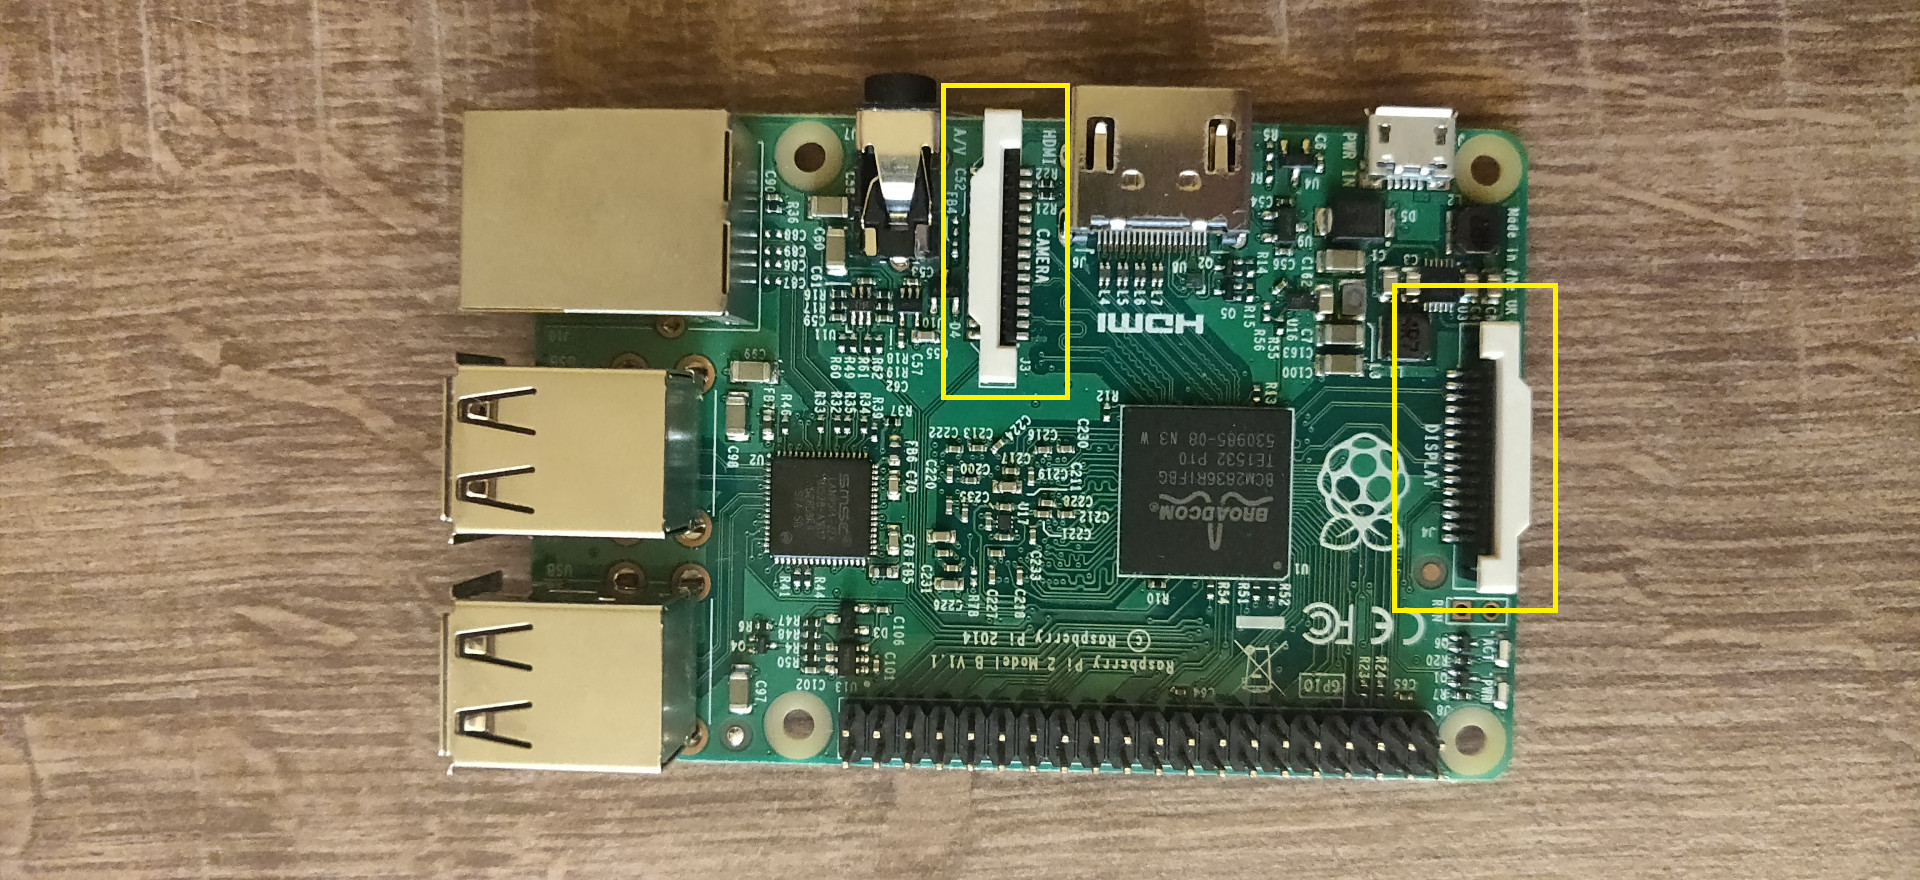
\includegraphics[width=0.95\textwidth, height=0.45\textwidth]{resources/Manual_Connections.jpg}
	\caption{Display and camera connections}
\end{figure}

When making the connection, make sure the pins on the ribbon cable match the pins on the port. Additionally,
the \(5V\) and \(GND\) pins on the display need to be connected to pins \(4\) and \(6\) respectively, on the Raspberry Pi.
Please refer to \url{https://www.raspberrypi.com/documentation/computers/raspberry-pi.html} in order to assess
the boards GPIO pinout.

\begin{figure}[H]
	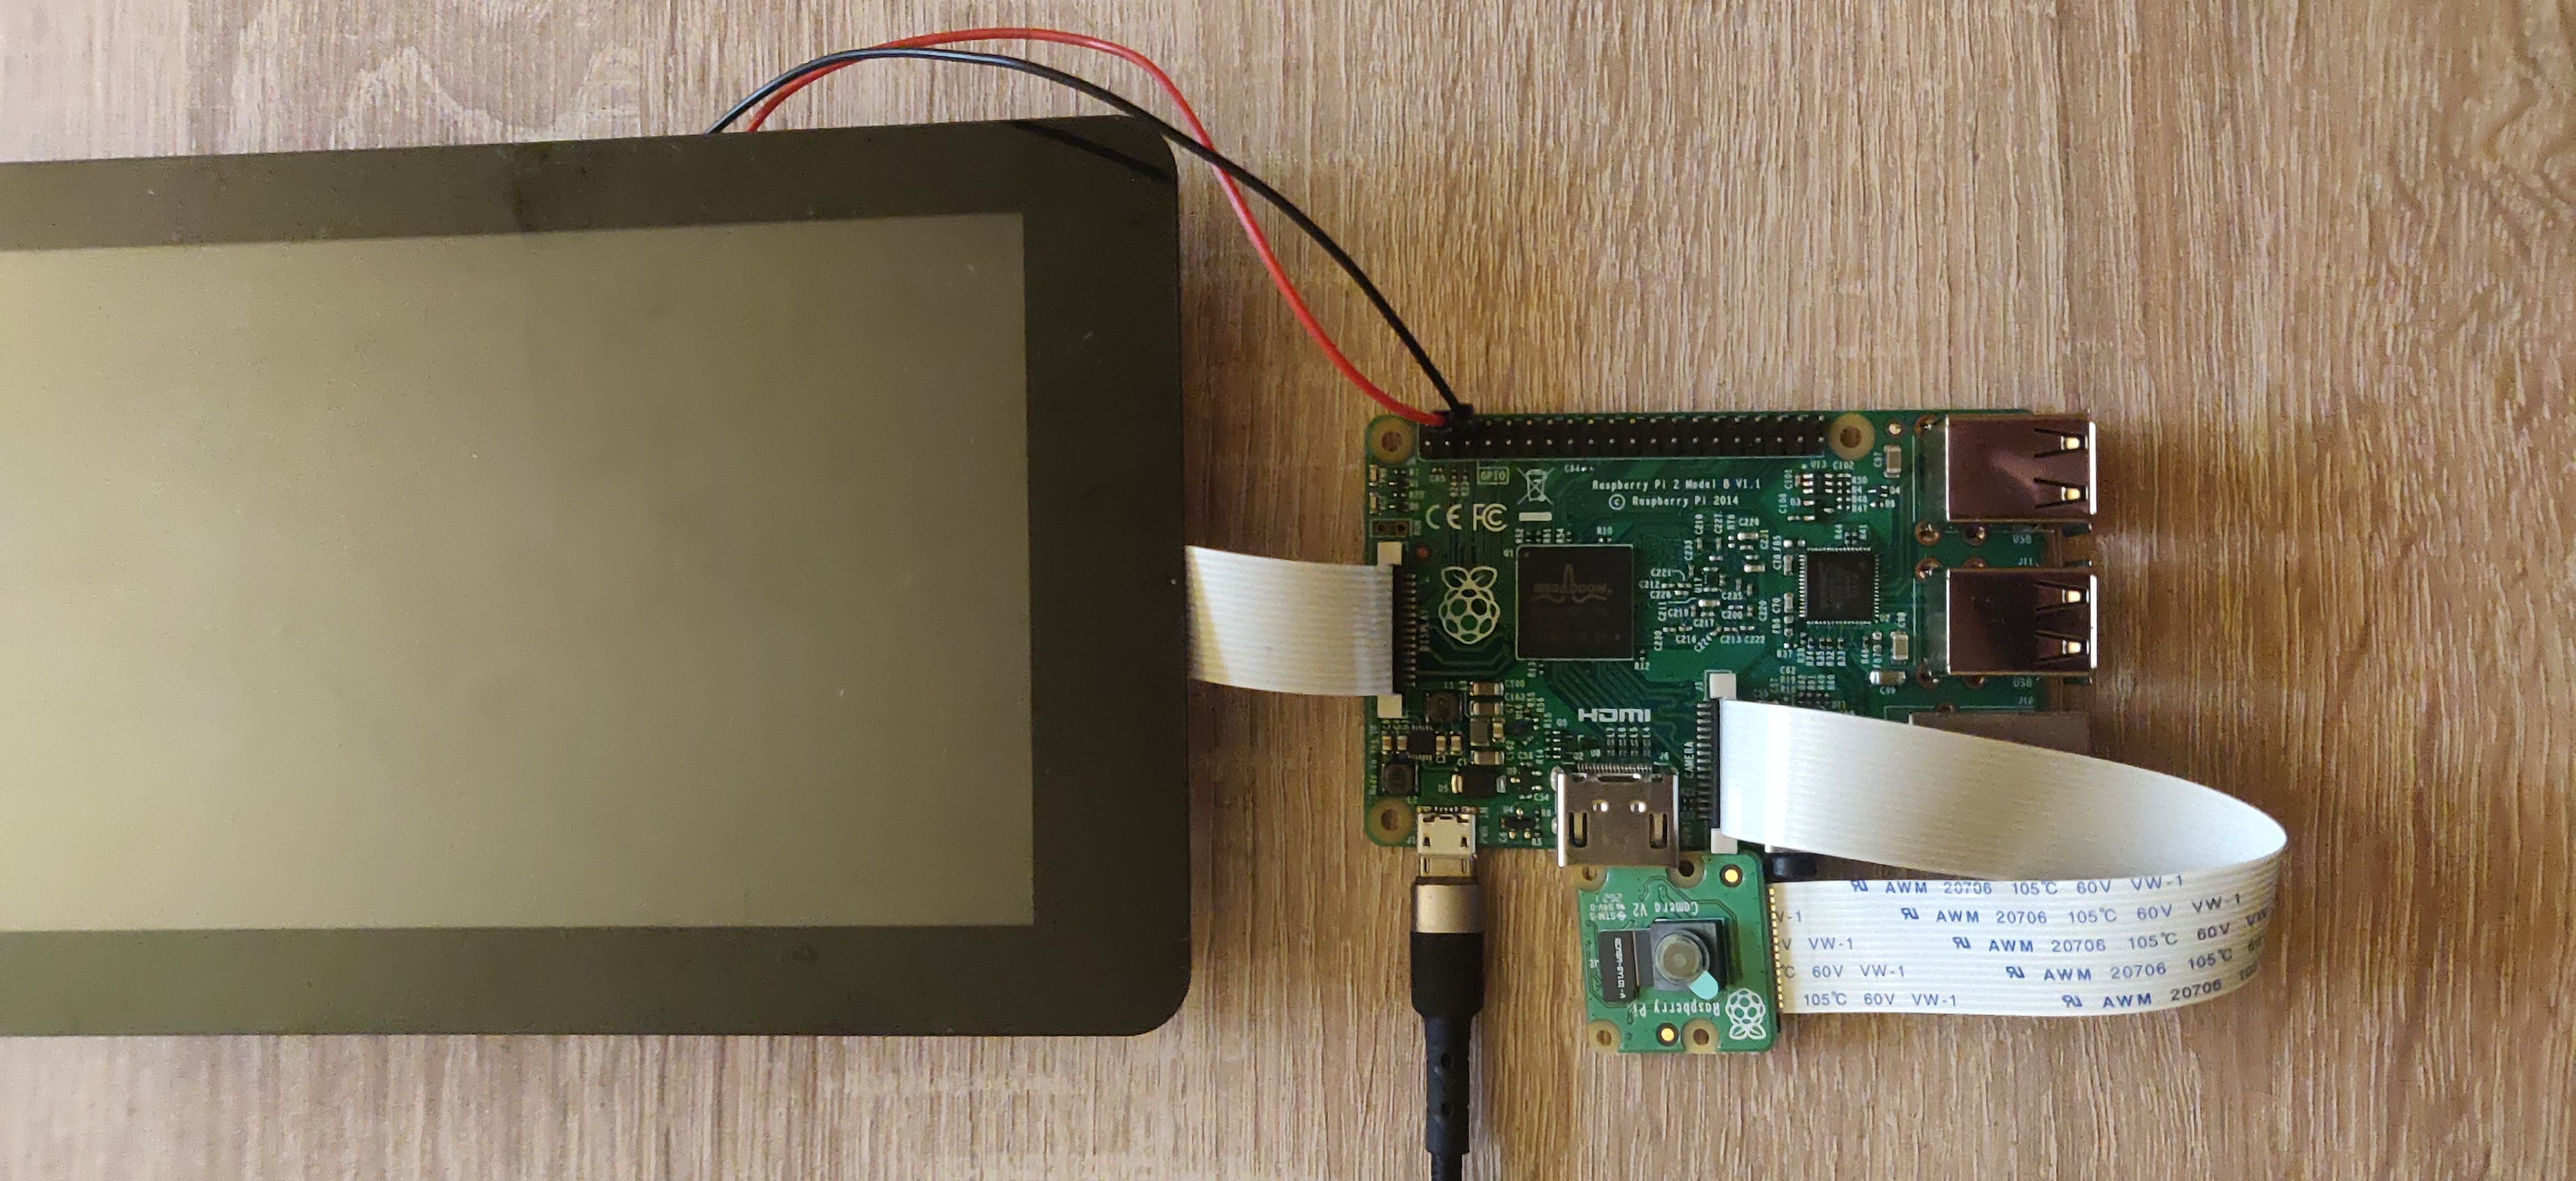
\includegraphics[width=0.95\textwidth, height=0.45\textwidth]{resources/Manual_Setup.jpg}
	\caption{Final setup}
\end{figure}

After all connections are made, the Raspberry Pi can be plugged in. The camera and display need to be enabled
using either the \verb|Preferences| menu or the \verb|raspi-config| utility, depending on the operating system.
An example can be consulted at the following address:
\url{https://techoverflow.net/2019/07/23/how-to-enable-raspberry-pi-camera-using-raspi-config/}.

Additionally, the board can be secured to the display, in order to help with the safety and portability of the
entire setup.

\section{Installation}

After installing \verb|git| or \verb|zip| on the system, copy the source code from
\url{https://gitlab.upt.ro/victor.toporan/ISP_Demo}

Upon cloning the repository, navigate to the source directory and use the \verb|dependencies.sh| script as superuser,
in order to install all required dependencies, or install them manually, using the systems package manager:
\begin{code}
	\begin{lstlisting}
    cd ISP_Demo
    sudo ./dependencies.sh
    \end{lstlisting}
	or
	\begin{lstlisting}
    sudo apt-get install g++
    sudo apt-get install cmake
    sudo apt-get install qt5-default
    sudo apt-get install libopencv-dev
    \end{lstlisting}
\end{code}

After that, use the \verb|install.sh| script, or compile manually, in order to build the executable and create
a desktop shortcut.

\begin{code}
	\begin{lstlisting}
    ./install.sh
    \end{lstlisting}
	or
	\begin{lstlisting}
    cd src
    cmake -H. -Bbuild
    cd build
    make all
    \end{lstlisting}
\end{code}

If the application was built manually, the executable will have the name \verb|ISP_Demo.exe|.
Upon completion, if the install script was used or a shortcut was manually created, navigate to the desktop and
run the application.

\pagebreak
\section{User Interface}

Opening the application, the following user interface will be shown:
\begin{figure}[H]
	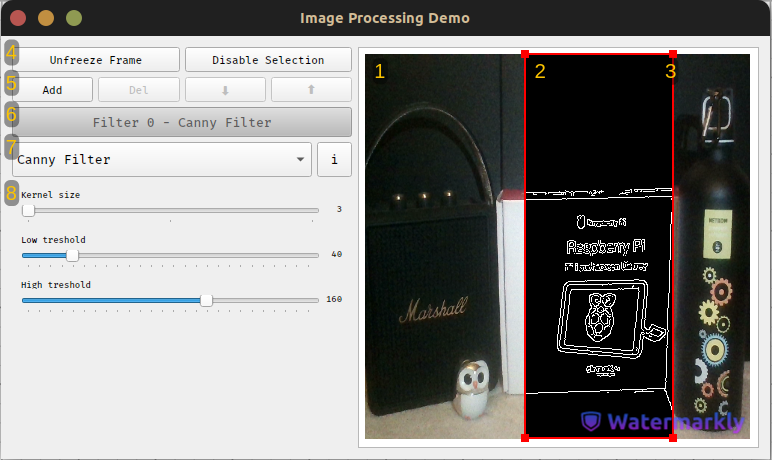
\includegraphics[width=0.95\textwidth, height=0.5\textwidth]{resources/Manual_Outline.jpg}
	\caption{User Interface Overview}
\end{figure}

It can be separated into the following subsections:
\begin{enumerate}
	\item Viewport - the resulting image, after all filters are applied, will be shown here.
	\item Region of interest - any given filter will be applied only within its designated ROI.
	\item ROI anchors - used to resize the region of interest.
	\item Miscellaneous - used to pause the frame capture and disable the ROI selection.
	\item Filter management - used to add, delete or change a filters application order.
	\item Filter layout - used to chose the active ROI and preview filter application order.
	\item Filter selection - used to change the currently applied filter, as well as provide
	      information about parameters.
	\item Parameter management - used to tweak filter parameters in order to change resulting image.
\end{enumerate}

\pagebreak
\section{Components}

The following components were used in the development of this project, and are included in the demo package:
\begin{enumerate}
	\item Raspberry Pi Model B - 1.5GHz Quad-core CPU and 4GB LPDDR4 RAM.
	\item Raspberry Pi Camera Module V2.1 - 8 megapixel Sony IMX219 image sensor, supporting 1080p capture at 30FPS.
	      Version 2 was discontinued, version 3 is recommended for future implementations.
	\item Raspberry Pi 7" Touchscreen Display - 800 x 480, powered through the development board.
\end{enumerate}

Bellow is a list of possible acquisition sites, if the need arises for the project to be replicated. Prices
may vary in accordance to currency exchange rates.

\newcommand{\raspioptimus}{https://www.optimusdigital.ro/ro/placi-raspberry-pi/11524-raspberry-pi-4-model-b-8gb-765756931199.html}
\newcommand{\raspipihut}{https://thepihut.com/products/raspberry-pi-4-model-b?variant=41005997392067}
\newcommand{\raspiamazonfirst}{https://www.amazon.com/Raspberry-Pi-4-4G-Model/dp/B081YD3VL5}
\newcommand{\raspiamazonsecond}{https://www.amazon.com/Raspberry-Model-2019-Quad-Bluetooth/dp/B07TC2BK1X?th=1}
\newcommand{\camerapihut}{https://thepihut.com/products/raspberry-pi-camera-module-3}
\newcommand{\displaypihut}{https://thepihut.com/products/official-raspberry-pi-7-touchscreen-display}
\newcommand{\displayamazon}{https://www.amazon.com/WIMAXIT-Raspberry-Monitor-1024x600-Raspbian/dp/B0932CX42D?ref_=ast_sto_dp}
\begin{longtable}[H]{|>{\cellcolor{white}}m{3cm}|m{3cm}|m{2.5cm}|>{\raggedleft\arraybackslash}m{4.5cm}|}
	\hiderowcolors
	\caption{Components acquisition details\label{tb:compoenntsEn}}                                                                                    \\
	\hline
	Component              & Link                                    & Price (RON) & Observations                                                      \\
	\hline
	\endfirsthead

	\hline
	\multicolumn{4}{|c|}{Continuation of Table \ref{tb:compoenntsEn}}                                                                                  \\
	\hline
	Component              & Link                                    & Price (RON) & Observations                                                      \\
	\hline
	\endhead

	\hline
	\endfoot

	\hline\hline
	\endlastfoot
	\showrowcolors

	\showrowcolors
	\hline
	Raspberry Pi 4 model B & \href{\raspioptimus}{OptimusDigital.ro} & 173 - 411   & Official Raspberry Pi retailer, all models available              \\
	                       & \href{\raspipihut}{thepihut.com}        & 200 - 425   & Official Raspberry Pi retailer, all models available              \\
	                       & \href{\raspiamazonfirst}{Amazon.com}    & 825 - 1015  & 8GB model                                                         \\
	                       & \href{\raspiamazonsecond}{Amazon.com}   & 600 - 805   & 4GB model                                                         \\
	\hline
	Raspberry Pi Camera V3 & \href{\camerapihut}{thepihut.com}       & 150         & Official Raspberry Pi retailer, previous versions discontinued    \\
	\hline
	7" Touchscreen Display & \href{\displaypihut}{thepihut.com}      & 385         & Official Raspberry Pi retailer, includes all required accessories \\
	                       & \href{\displayamazon}{Amazon.com}       & 375         & Includes standing mount                                           \\
\end{longtable}

If any component is to be exchanged for a different model, due to performance or cost, it is recommended that
the project configuration is updated accordingly.

\chapter{Manual de utilizare}

Deoarece aplicația a fost concepută ca o demonstrație practică, menită pentru prezentarea pe o placă Raspberry Pi,
acest manual prezintă informația necesară configurării integrale a sistemului. Acesta prezintă ghidul de
asamblare pentru placa Raspberry Pi, instrucțiuni pentru compilarea și instalarea aplicației și o prezentare
de ansamblu asupra interfeței grafice.

\section{Configurare Raspberry Pi}

\begin{figure}[H]
	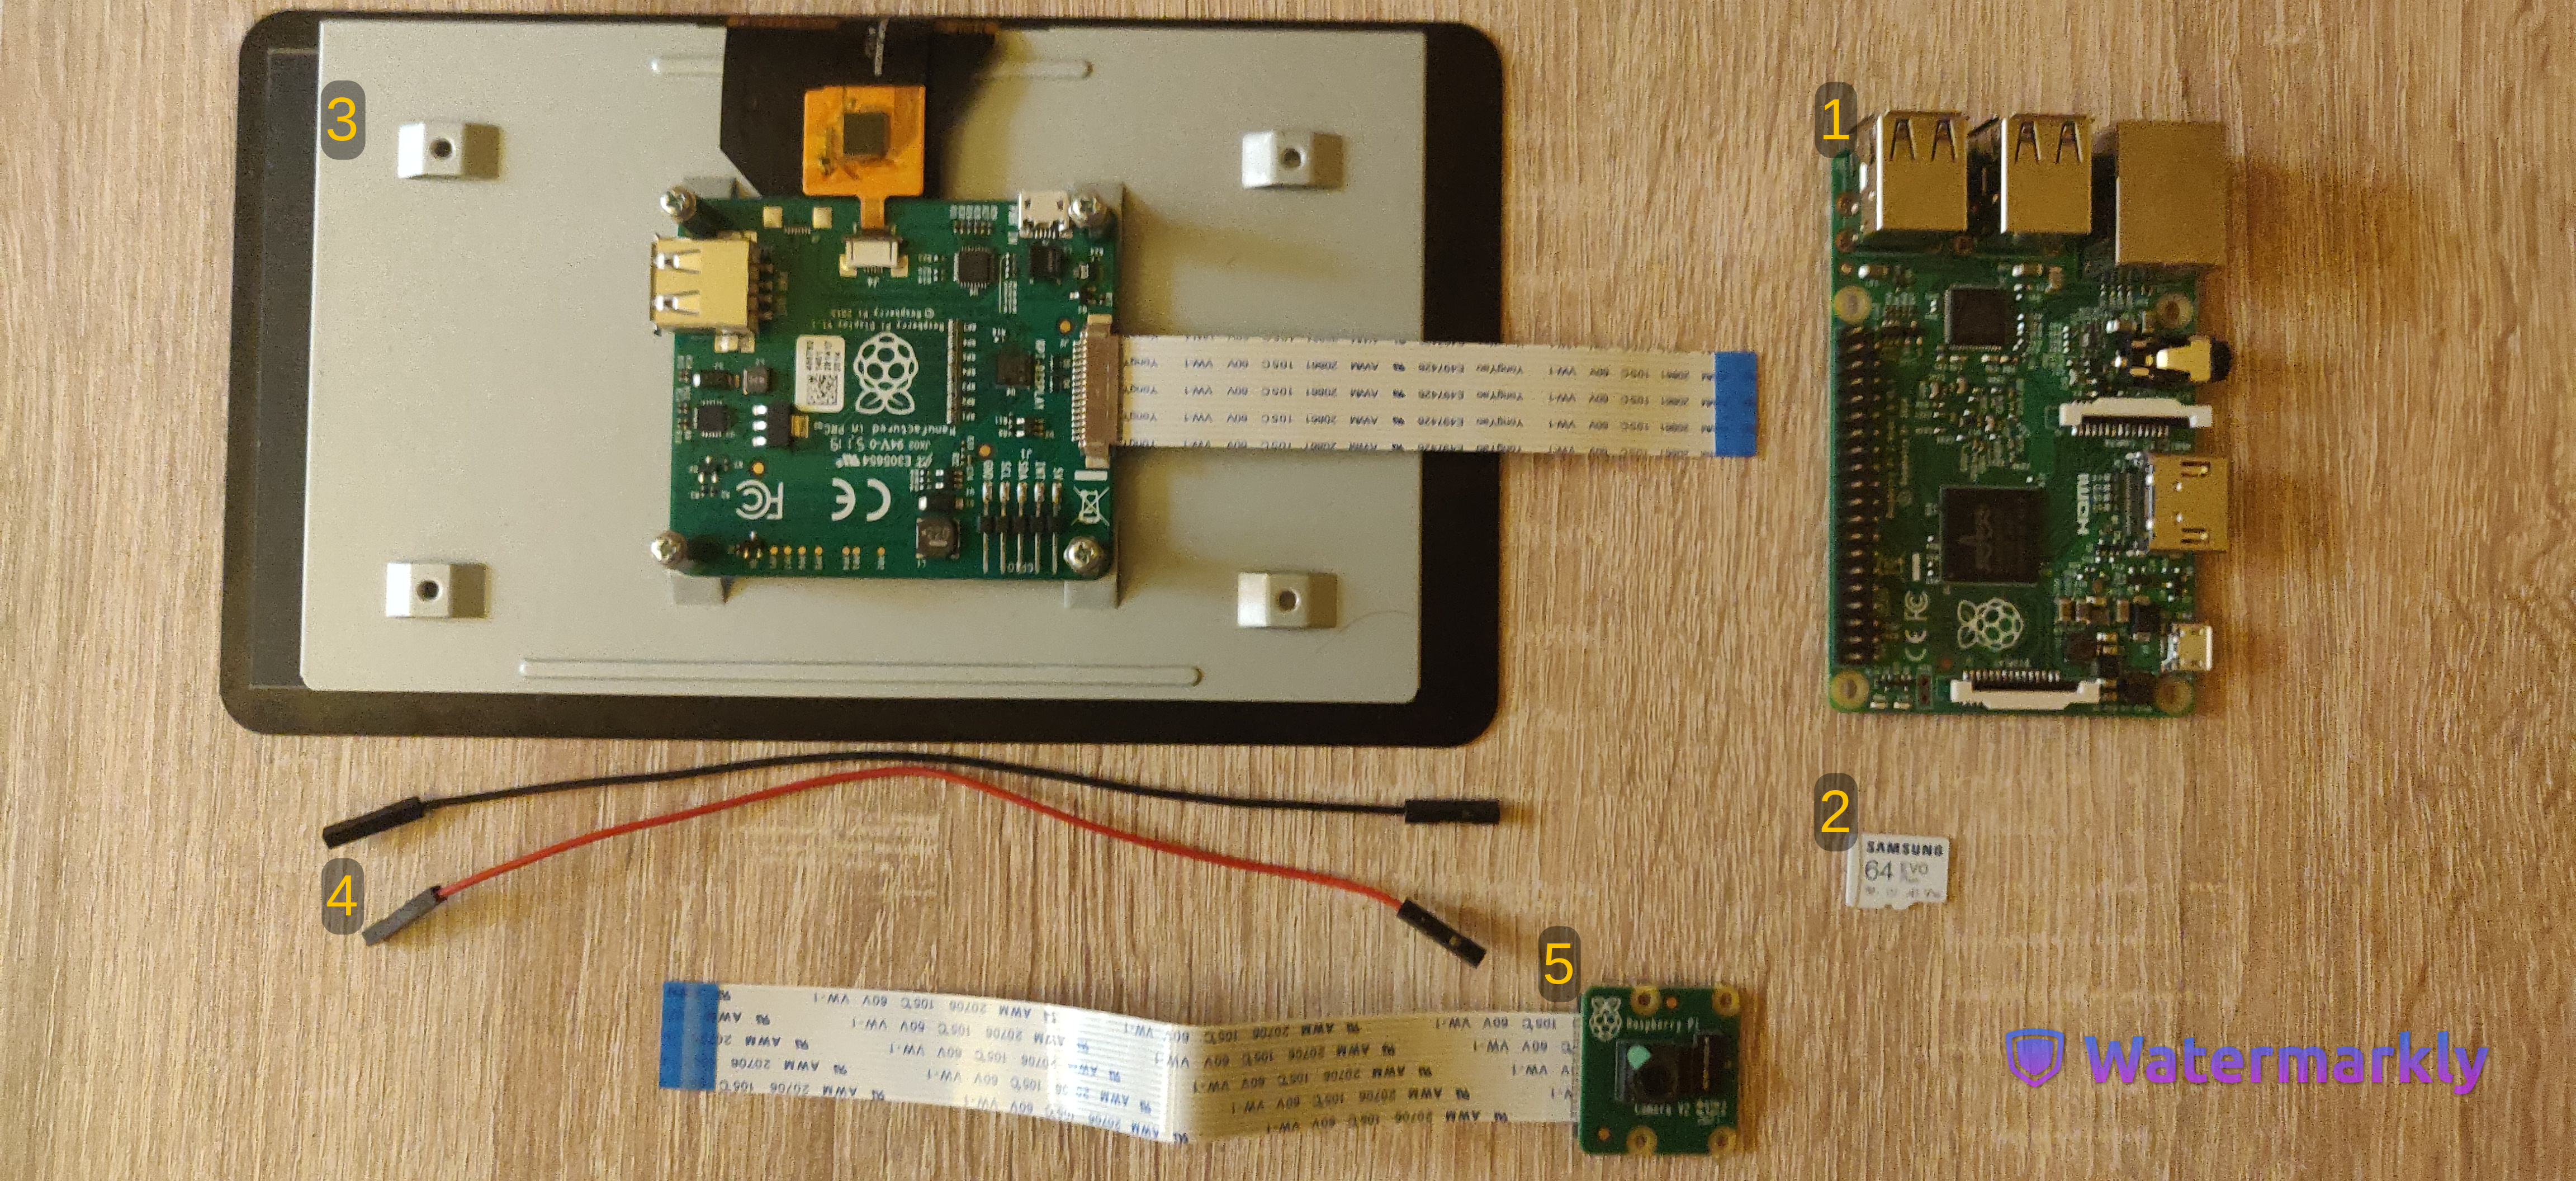
\includegraphics[width=0.95\textwidth, height=0.5\textwidth]{resources/Manual_Components.jpg}
	\caption{Componente necesare}
\end{figure}

Aceste componente sunt, în ordine:
\begin{enumerate}
	\item Placă de dezvoltare Raspberry Pi.
	\item Card SD pentru stocarea sistemului de operare.
	\item Display Raspberry Pi, cu cablu de conectare.
	\item Fire de curent pentru display.
	\item Camera Raspberry Pi, cu cablu de conectare.
\end{enumerate}

Înainte de a conecta componentele, un sistem de operare valid, bazat pe Debian, trebuie instalat pe cardul
SD. Această procedură este descrisă în documentația oficială a Raspberry Pi:
\url{https://www.raspberrypi.com/documentation/computers/getting-started.html#installing-the-operating-system}.

Următoarele porturi sunt destinate conexiunilor pentru display, respectiv cameră:

\begin{figure}[H]
	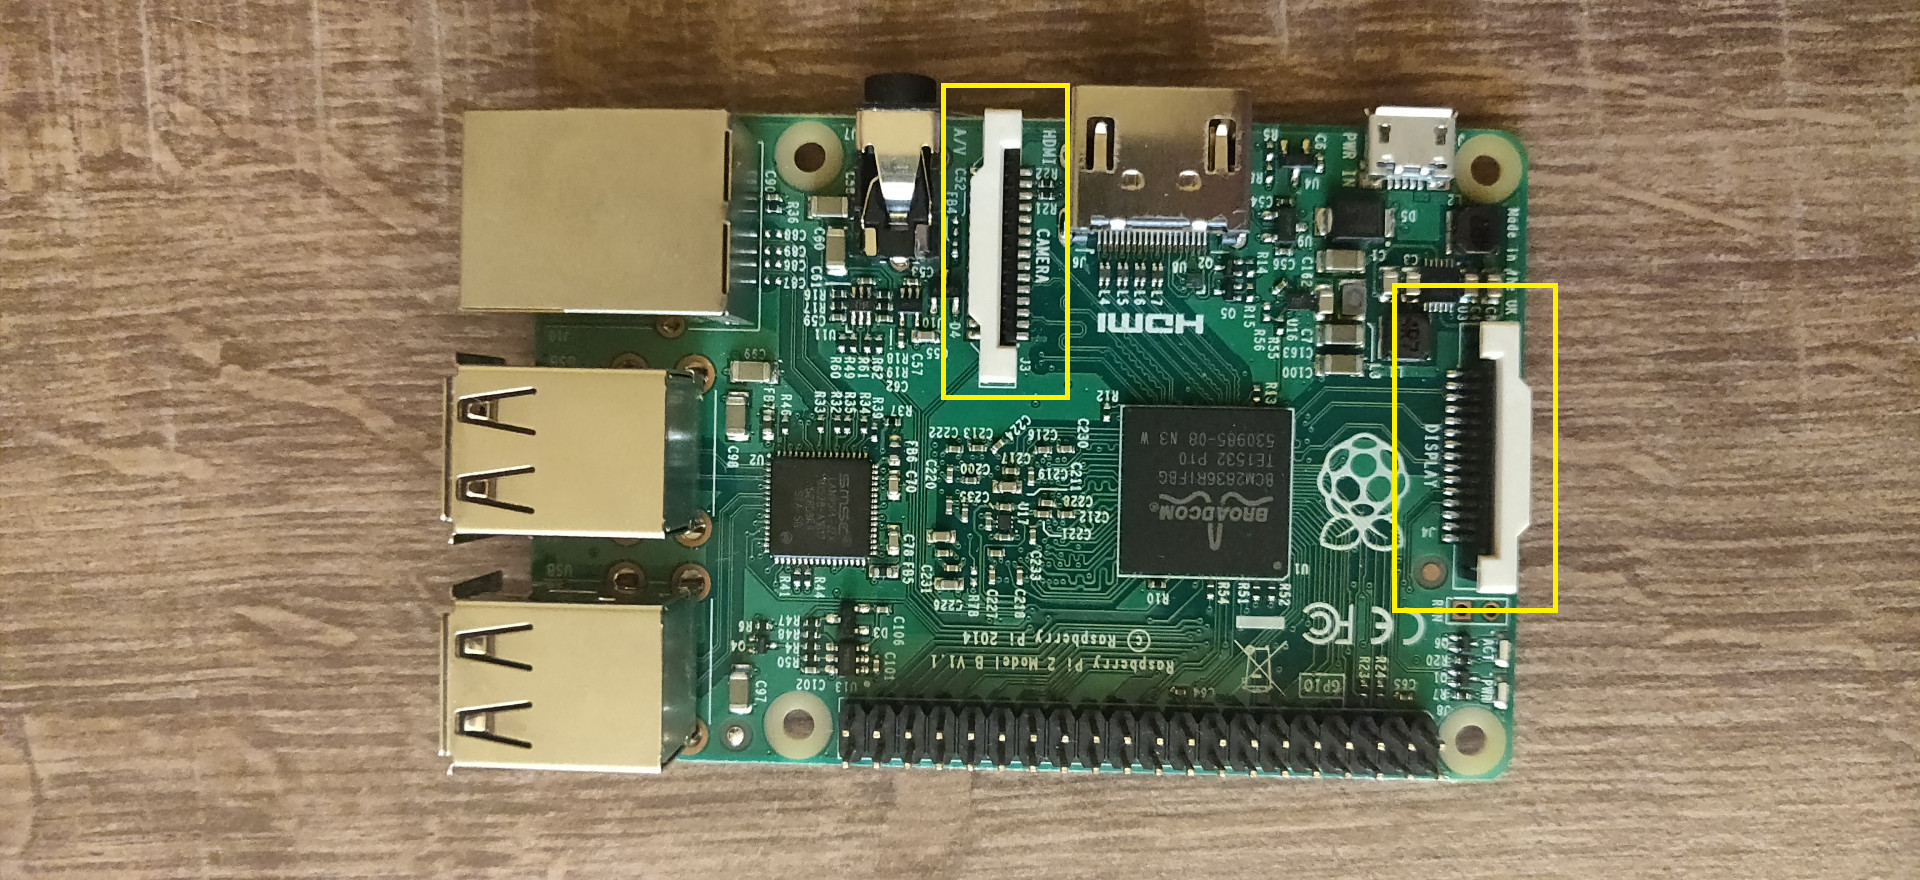
\includegraphics[width=0.95\textwidth, height=0.45\textwidth]{resources/Manual_Connections.jpg}
	\caption{Conexiuni display și cameră}
\end{figure}

Pentru aceste conexiuni, este necesar ca pinii de pe cablul de conectare să fie aliniați cu pinii fiecărui
port și pinii marcați \(5V\) și \(GND\) de pe display să fie conctați la pinii \(4\), respectiv \(6\) de
pe Raspberry Pi. Pentru a vizualiza configurația pinilor GPIO de pe placă, poate fi folosită documentația
oficială: \url{https://www.raspberrypi.com/documentation/computers/raspberry-pi.html}

\begin{figure}[H]
	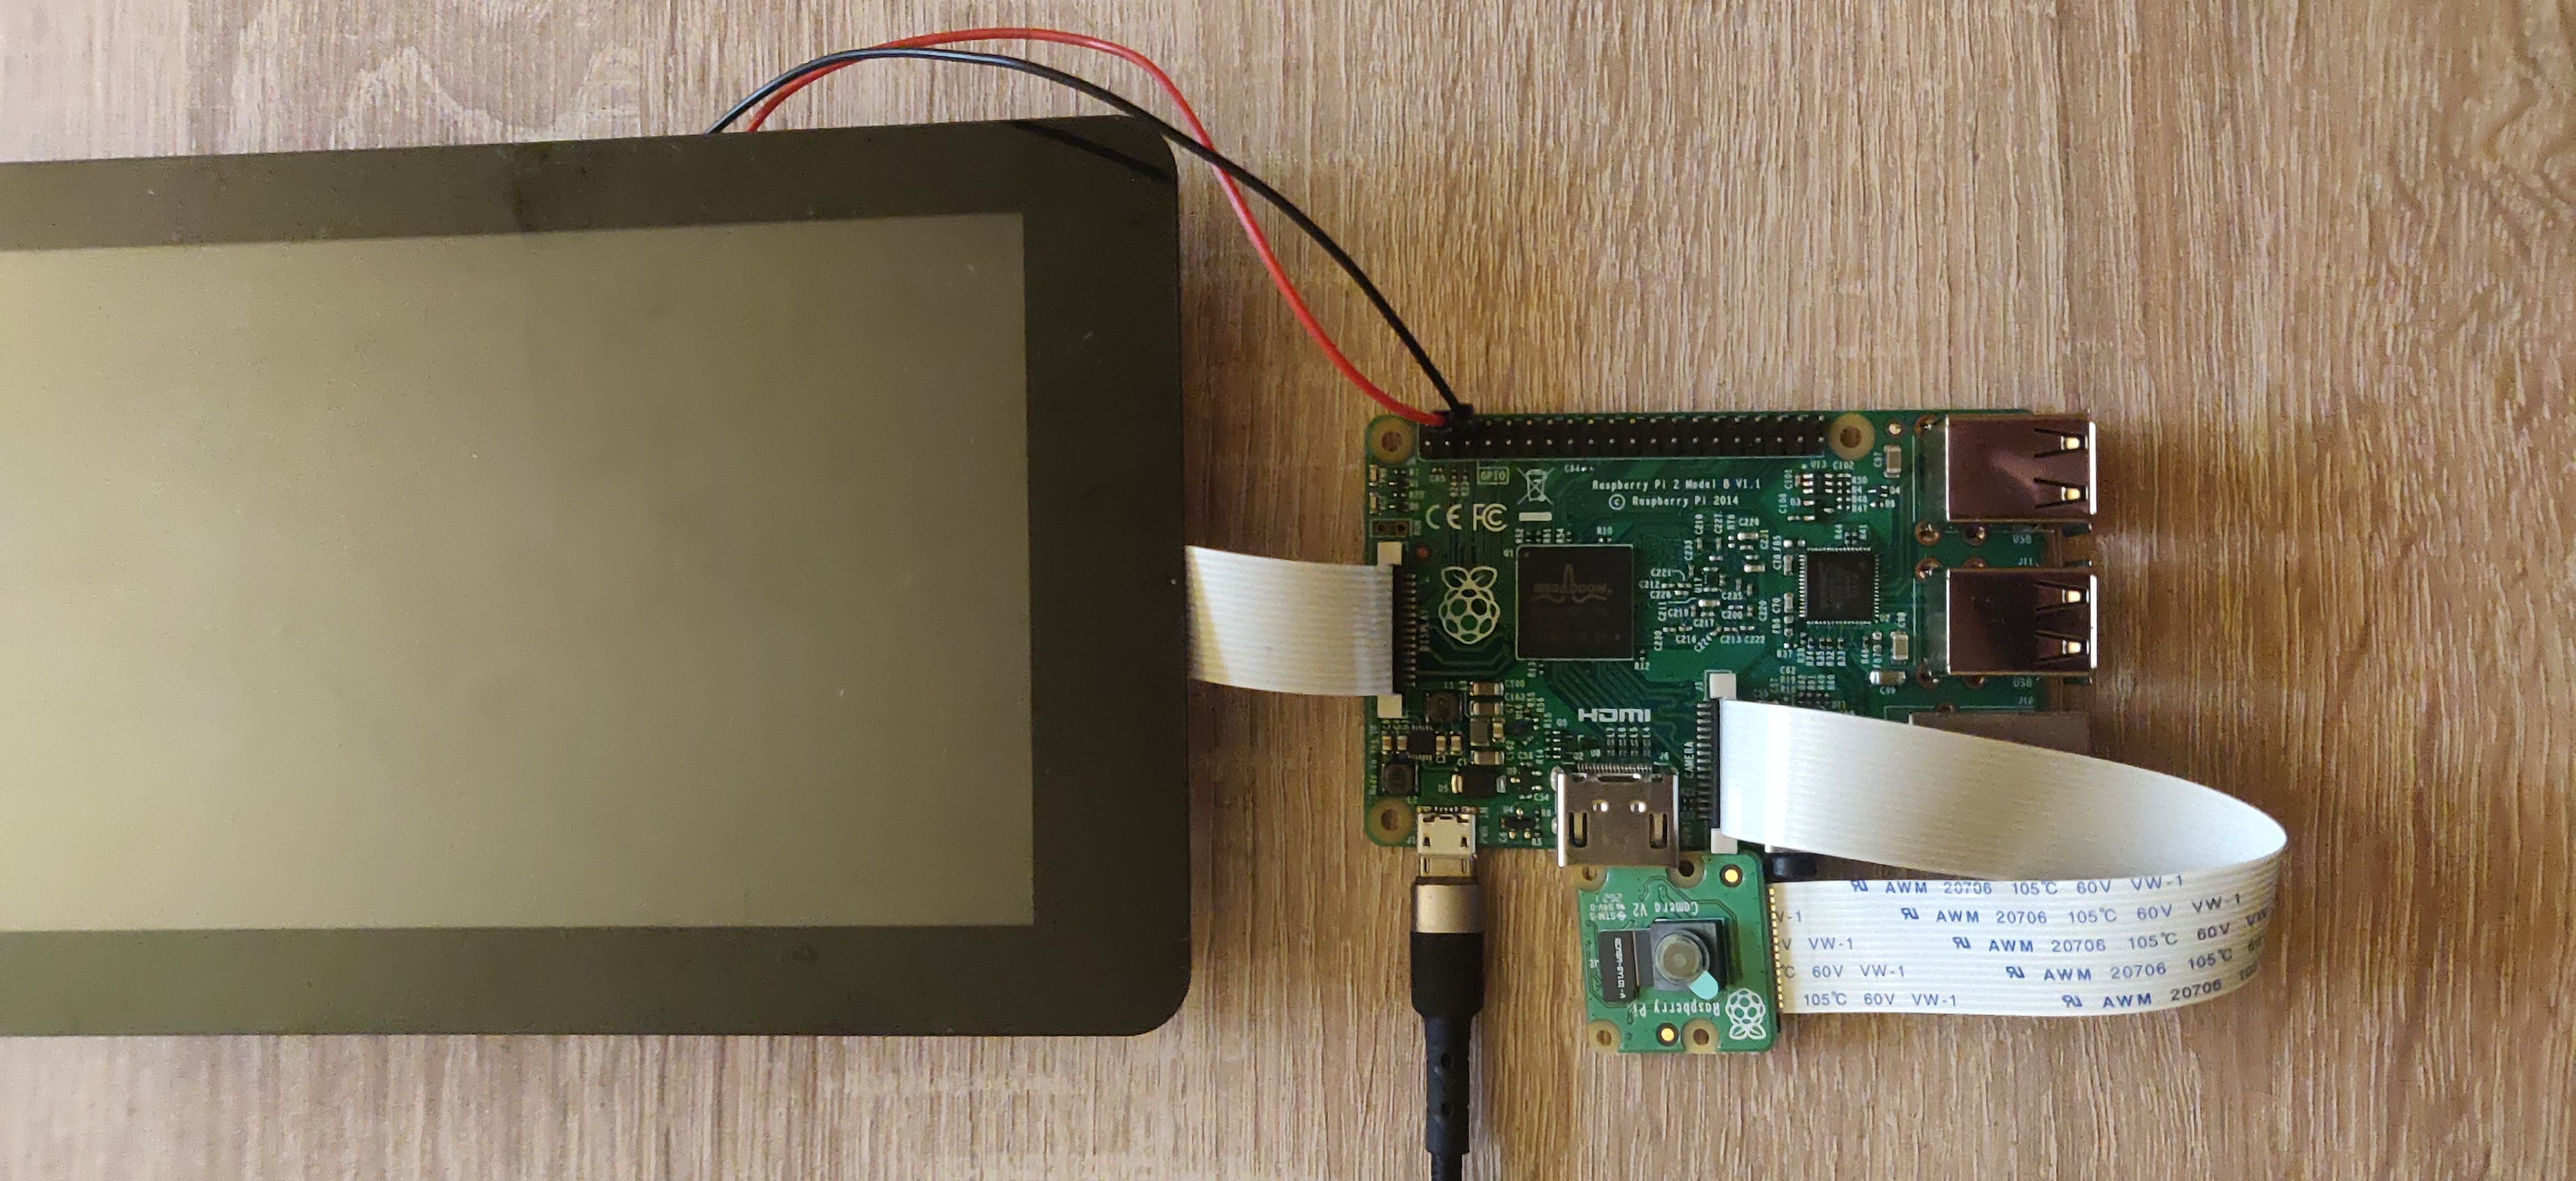
\includegraphics[width=0.95\textwidth, height=0.45\textwidth]{resources/Manual_Setup.jpg}
	\caption{Asamblare completă}
\end{figure}

După legarea tuturor conexiunilor, placa Raspberry Pi poate fi legată la o sursă de curent. Camera și display-ul
vor trebui activate, fie prin intermediul meniului de \verb|Preferințe| sau prin utilitarul \verb|raspi-config|,
în funcție de sistemul de operare. Această procedură poate este descrisă la următoarea adresă:
\url{https://techoverflow.net/2019/07/23/how-to-enable-raspberry-pi-camera-using-raspi-config/}.

Suplimentar, placa poate fi montată pe display, dacă se dorește securizarea acesteia și reducerea
spațiului ocupat de întregul sistem.

\section{Instalare}

După instalarea utilitarelor \verb|git| sau \verb|zip| pe sistem, codul sursă poate fi accesat la următoarea adresă:
\url{https://gitlab.upt.ro/victor.toporan/ISP_Demo}

Odată ce repository-ul a fost clonat, script-ul \verb|dependencies.sh| poate fi rulat ca superuser, pentru
a instala toate dependințele necesare. Alternativ, acestea pot fi instalate manual, folosind package
manager-ul specific sistemului de operare folosit:

\begin{code}
	\begin{lstlisting}
    cd ISP_Demo
    sudo ./dependencies.sh
    \end{lstlisting}
	sau
	\begin{lstlisting}
    sudo apt-get install g++
    sudo apt-get install cmake
    sudo apt-get install qt5-default
    sudo apt-get install libopencv-dev
    \end{lstlisting}
\end{code}

După instalarea tuturor dependințelor, aplicația poate fi instalată folosind script-ul \verb|install.sh|, care
va crea și un shortcut, sau poate fi compilată manual, rezultatul fiind executabilul \verb|ISP_Demo.exe|.

\begin{code}
	\begin{lstlisting}
    ./install.sh
    \end{lstlisting}
	sau
	\begin{lstlisting}
    cd src
    cmake -H. -Bbuild
    cd build
    make all
    \end{lstlisting}
\end{code}

În cazul în care un shortcut a fost creat, fie prin utilizarea script-ului, fie manual, aplicația va putea
fi accesată direct din desktop, prin intermediul acestuia.

\pagebreak
\section{Interfață Grafică}

Următoarea interfață va fi afișată la pornirea aplicației:
\begin{figure}[H]
	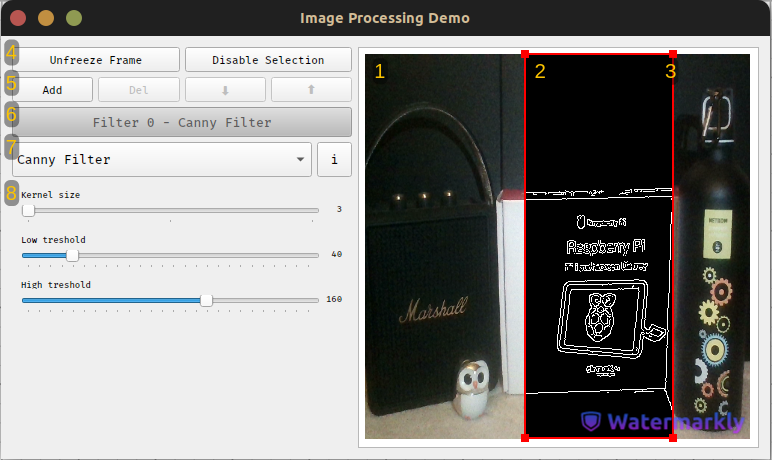
\includegraphics[width=0.95\textwidth, height=0.5\textwidth]{resources/Manual_Outline.jpg}
	\caption{Diviziunile interfeței grafice}
\end{figure}

Aceasta este împărțită în următoarele secțiuni:
\begin{enumerate}
	\item Viewport - afișează imaginea finală, după aplicarea tuturor filtrelor.
	\item Regiune de interes - fiecare filtru va fi aplicat doar în interiorul regiunii desemnate.
	\item Puncte de ancorare - folosite pentru a modifica aria regiunii de interes.
	\item Diverse - butoane folosite pentru a opri stream-ul video și pentru a dezactiva selecția regiunilor de interes.
	\item Management al filtrelor - butoane folosite pentru adăugarea, ștergerea sau schimbarea poziției unui filtru.
	\item Dispunerea filtrelor - butoane folosite pentru a selecta regiunea activă și pentru a vizualiza ordinea de aplicare.
	\item Selectarea filtrului - meniu folosit pentru a selecta filtrul curent și pentru a vizualiza informații despre acesta.
	\item Management al parametrilor - slider-e folosite pentru a ajusta parametrii unui filtru, în timp real.
\end{enumerate}

\pagebreak
\section{Componente}

Următoarele componente au fost folosite în realizarea acestui proiect și sunt incluse în pachetul pentru prezentare:
\begin{enumerate}
	\item Raspberry Pi Model B - 1.5GHz Quad-core CPU și 4GB LPDDR4 RAM.
	\item Raspberry Pi Camera Module V2.1 - 8 megapixel Sony IMX219, ce permite captură 1080p la 30FPS.
	      Versiunea 2 a fost scoasă din producție, versiunea 3 este recomandată pentru viitoare implementări.
	\item Raspberry Pi 7" Touchscreen Display - 800 x 480, powered through the development board.
\end{enumerate}

Lista următoare prezintă posibile modalități de achiziție, în cazul în care se dorește replicarea proiectului.
Prețurile pot varia în funcție de cursul valutar.

\begin{longtable}[H]{|>{\cellcolor{white}}m{3cm}|m{3cm}|m{2.5cm}|>{\raggedleft\arraybackslash}m{4.5cm}|}
	\hiderowcolors
	\caption{Detalii pentru achiziția componentelor\label{tb:compoenntsRo}}                                                                                         \\
	\hline
	Componentă             & Link                                    & Preț (RON) & Observații                                                                      \\
	\hline
	\endfirsthead

	\hline
	\multicolumn{4}{|c|}{Continuare a Tabelului \ref{tb:compoenntsRo}}                                                                                              \\
	\hline
	Componentă             & Link                                    & Preț (RON) & Observații                                                                      \\
	\hline
	\endhead

	\hline
	\endfoot

	\hline\hline
	\endlastfoot
	\showrowcolors

	\showrowcolors
	\hline
	Raspberry Pi 4 model B & \href{\raspioptimus}{OptimusDigital.ro} & 173 - 411  & Retailer official Raspberry Pi, toate modelele disponibile                      \\
	                       & \href{\raspipihut}{thepihut.com}        & 200 - 425  & Retailer official Raspberry Pi, toate modelele disponibile                      \\
	                       & \href{\raspiamazonfirst}{Amazon.com}    & 825 - 1015 & Model 8GB                                                                       \\
	                       & \href{\raspiamazonsecond}{Amazon.com}   & 600 - 805  & Model 4GB                                                                       \\
	\hline
	Raspberry Pi Camera V3 & \href{\camerapihut}{thepihut.com}       & 150        & Retailer official Raspberry Pi, versiunile anterioare sunt scoade din producție \\
	\hline
	7" Touchscreen Display & \href{\displaypihut}{thepihut.com}      & 385        & Retailer official Raspberry Pi, include toate accesoriile necesare              \\
	                       & \href{\displayamazon}{Amazon.com}       & 375        & Include stand vertical                                                          \\
\end{longtable}

Dacă o componentă este înlocuită cu un alt model, din motive de performanță sau cost, este recomandat ca și
configurația aplicației să fie modificată în concordanță.

